\documentclass[10pt]{beamer}
%\documentclass[10pt, handout]{beamer}
%\usetheme{Madrid}
%\newlength{\pageheight}
%\setlength{\pageheight}{10cm}
%\usepackage{handoutWithNotes}
%\pgfpagesuselayout{2 on 1 with notes landscape}[a4paper,border shrink=5mm]

\usepackage[utf8]{inputenc}
\usepackage{dirtytalk}
\usepackage{amsmath}
\usepackage{amsfonts}
\usepackage{general}
\usepackage{minted}
\usepackage{booktabs}

\usepackage[nott]{inconsolata}

\DeclareMathOperator*{\argmax}{arg\,max}
%\DeclareMathOperator*{\argmin}{arg\,min}
\DeclareMathOperator*{\argmin}{\arg\min}

\definecolor{darkgreen}{rgb}{0.0, 0.5, 0.0}

\usepackage{pgf}
\usepackage{tikz}
\usetikzlibrary{arrows,automata}
\beamertemplatenavigationsymbolsempty

\addtobeamertemplate{title page}{
\includegraphics[scale=.5]{{../Images/UNAH-version-horizontal.png}}} %\hfill 
\includegraphics[scale=.3]{fabstracts2.png}}{}


%\titlegraphic{
%    \begin{tikzpicture}[overlay, remember picture]
%\node[at=(current page.north), anchor=north] {%
%    
\includegraphics[width=0.2\textwidth]{University_of_Pittsburgh_seal.png}
%    
\includegraphics[width=0.35\textwidth]{fabstracts.png}
%        };
%    \end{tikzpicture}
%}

\title{Text mining the arXiv with LLMs}
\subtitle{Un diccionario de matemáticas generado automáticamente}
\author{Luis Berlioz\\
\texttt{luis.berlioz@unah.edu.hn}}
\institute{Universidad Nacional Autónoma de Honduras}

\newcommand{\arxiv}{arXiv}
\begin{document}
\begin{frame}
\titlepage
\end{frame}


%%%%  FRAME  %%%%
\begin{frame}
    \frametitle{Objetivos}
    \begin{itemize}
        \item Extraer \emph{todos} los \textcolor<2>{red}{términos} matemáticos usados en la página \arxiv{} usando \textcolor<3>{red}{LLMs}.
            \note{Un termino matematico.\\
                No solo de arxiv, sino de cualquier literatura matematica}
            \begin{columns}
                \begin{column}{0.5\textwidth}
            \begin{center}
                
\includegraphics[width=0.6\textwidth]{../Images/ArXiv_logo_2022.svg.png}
            \end{center}
        \end{column}
        \begin{column}{0.5\textwidth}
            \begin{center}
                
\includegraphics[width=0.6\textwidth]{../Images/all_llm_logos.jpeg}
            \end{center}

        \end{column}
    \end{columns}
    \onslide<4>
        \item Organizar los términos en base a importancia y significado.  
            \note{importancia y significado no son muy especificos y esto es a proposito.}
    \end{itemize}
\end{frame}


%%%%  FRAME  %%%%
\begin{frame}[fragile]
    \frametitle{Origen de los Datos}
    \begin{itemize}
        \item arXiv permite descargar el codigo fuente de muchísimos artículos.
            \pause
        \item Algunos autores marcan sus definiciones con un ambiente de \emph{definition}
            \begin{minted}[linenos=true]{latex}
\begin{definition}
    Un Grupo es un monoide donde todo ...
\end{definition}
    \end{minted}
    \pause
\item Para identificar el término, usamos Wikipedia, Stacks Project, etc.
    \begin{columns}
        \begin{column}{0.4\textwidth}
            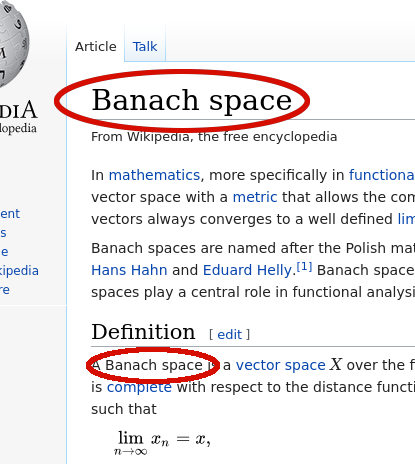
\includegraphics[width=0.9\textwidth]{../Images/wiki_thin_banach.png}
        \end{column}
        \pause
        \begin{column}{0.6\textwidth}
            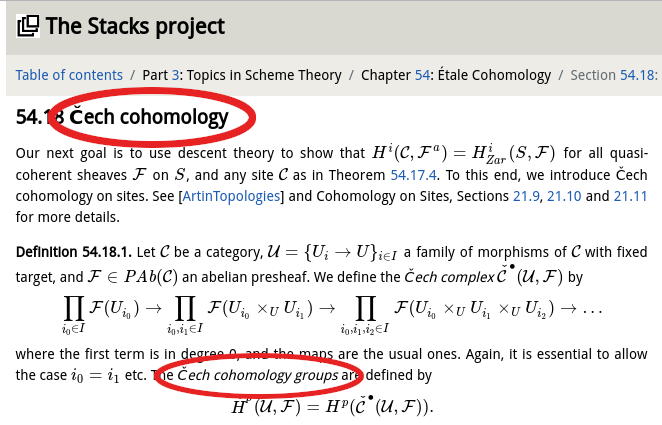
\includegraphics[width=0.8\textwidth]{../Images/stacks_defs.png}
        \end{column}
    \end{columns}

\end{itemize}
\end{frame}


%%%%  FRAME  %%%%
\begin{frame}
    \frametitle{Entrenando al Clasificador}
    Usando estos datos podemos entrenar \textbf{clasificador de secuencias} (Sequence Classifier). \pause Ejemplo tomado de \textcolor{blue}{arxiv.org/abs/0805.2034}
    \begin{center}
        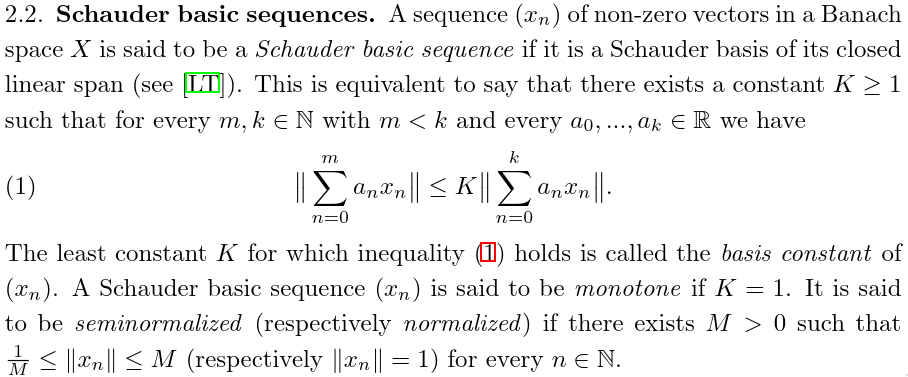
\includegraphics[width=0.7\textwidth]{../Images/def2.png}
    \end{center}
    \phantom{Luego podemos entrenar un \textbf{clasificador de tokenes}. Para encontrar el término que se está definiendo.}
\end{frame}

%%%%  FRAME  %%%%
\begin{frame}
    \frametitle{Entrenando al Clasificador}
    Usando estos datos podemos entrenar \textbf{clasificador de secuencias} (Sequence Classifier). Ejemplo tomado de \textcolor{blue}{arxiv.org/abs/0805.2034}
    \begin{center}
        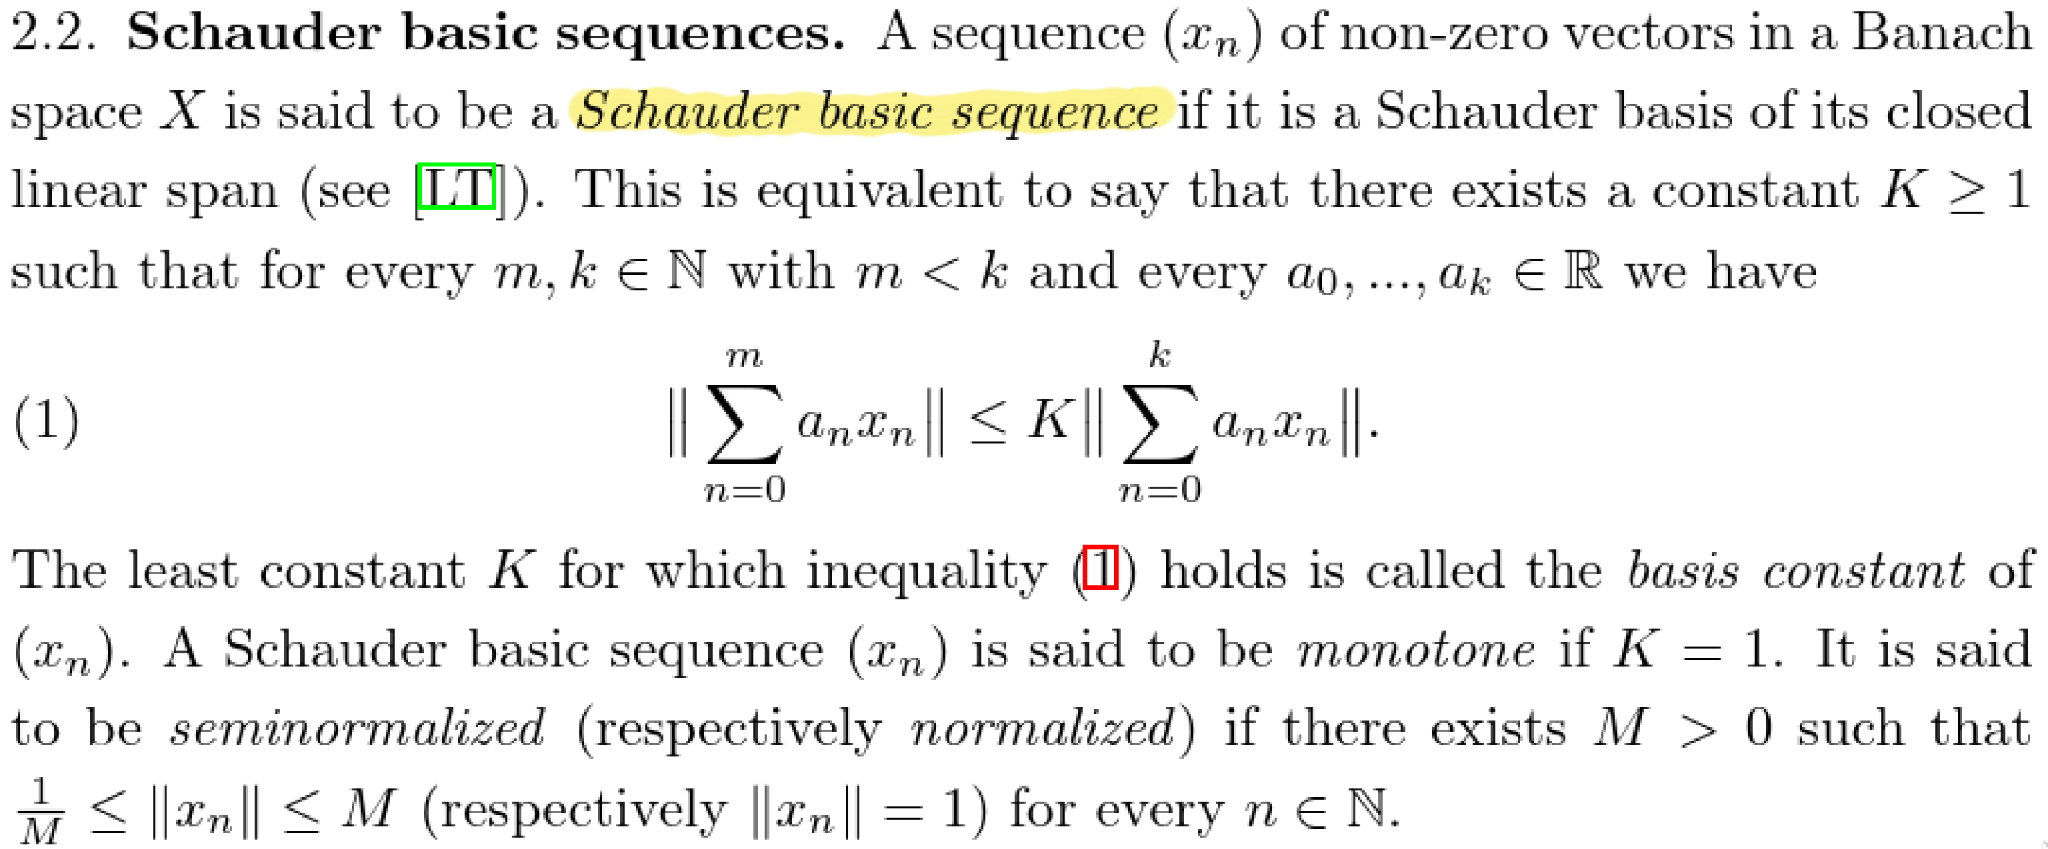
\includegraphics[width=0.7\textwidth]{../Images/def_highlighted.png}
    \end{center}
    Luego podemos entrenar un \textbf{clasificador de tokenes}. Para encontrar el término que se está definiendo.
\end{frame}

%%%%  FRAME  %%%%
\begin{frame}[containsverbatim]
    \frametitle{Un poquito de código}
    \framesubtitle{Entonando (finetuning) modelos pre-entrenado}
    \begin{minted}{python}
# IMPORTAMOS LAS LIBRERIAS DE HUGGINGFACE
from transformers import (AutoTokenizer,
                  AutoModelForSequenceClassification,
                  TFAutoModelForTokenClassification,
                  DataCollatorWithPadding,)

#checkpoint = "roberta-large"
#checkpoint = "bigscience/bloom-1b1"
checkpoint = "gpt2"

# ITERACIONES DE ENTRENAMIENTO (3 - 5)
for epoch in tqdm(range(epochs)):
    train_labels, train_predict, train_loss = \
    train(train_dataloader,
        optimizer, scheduler, device)
    ... ... ...
    \end{minted}
\end{frame}

%%%%  FRAME  %%%%
\begin{frame}
    \frametitle{Métricas y Resultados}
    \begin{columns}
        \begin{column}{0.3\textwidth}
            \begin{itemize}
                \item El desempeño de los LLMs es mejor.
                    \pause
                \item BERT es el mejor.
                    \pause
            \end{itemize}
        \end{column}
        \begin{column}{0.7\textwidth}
            \begin{center}
                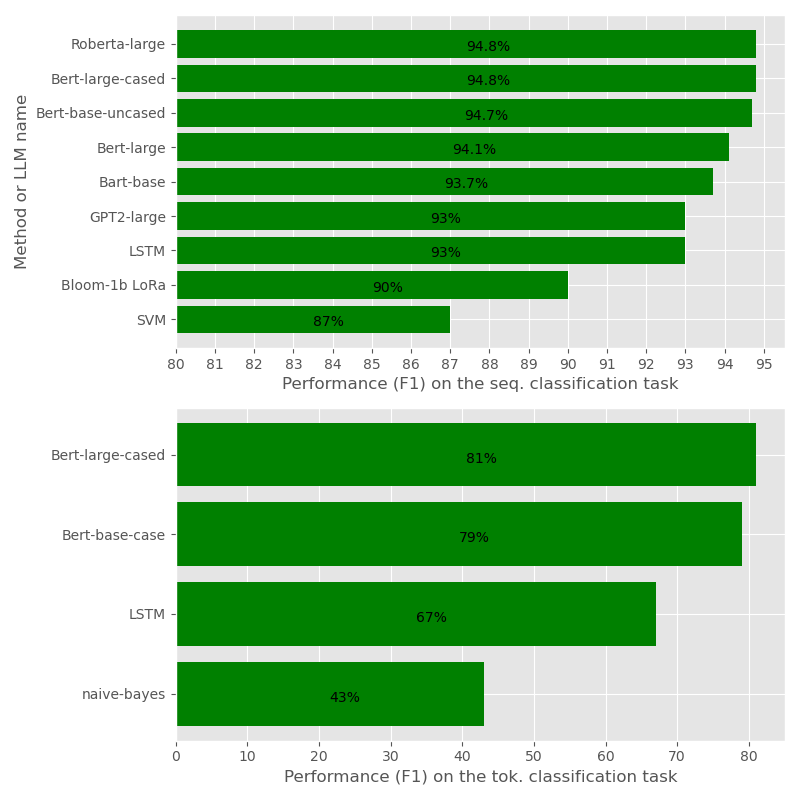
\includegraphics[width=0.9\textwidth]{../Images/taskbars.png}
            \end{center}
        \end{column}
    \end{columns}
\end{frame}


%%%%  FRAME  %%%%
\begin{frame}
    \frametitle{Visualizando los Resultados}
    \begin{columns}
        \begin{column}{0.4\textwidth}
        Términos con más de una palabra\\
            \begin{tabular}{lr}
                \toprule
                \textbf{Término} & \textbf{\#}  \\
                \midrule
full subcategory &  6,836 \\
weak solution &  4,926 \\
finitely generated &  3,791 \\
well defined &  3,476 \\
tensor product &  2,937 \\
simplicial complex &  2,610 \\
lie group &  2,578 \\
finite set &  2,341 \\
probability measure &  2,089 \\
banach space &  2,027 \\
borel measure &  1,999 \\
young diagram &  1,985 \\
non degenerate &  1,861 \\
moduli space &  1,848 \\
hilbert space &  1,795 \\
\bottomrule
            \end{tabular}
        \end{column}
        \begin{column}{0.6\textwidth}
            \begin{center}
                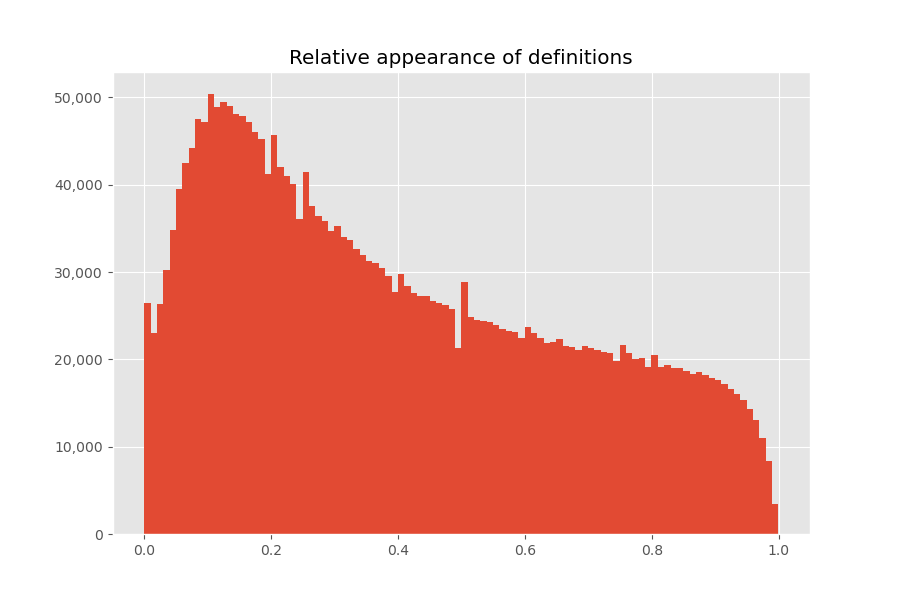
\includegraphics[width=0.95\textwidth]{../Images/rel_appe.png}

                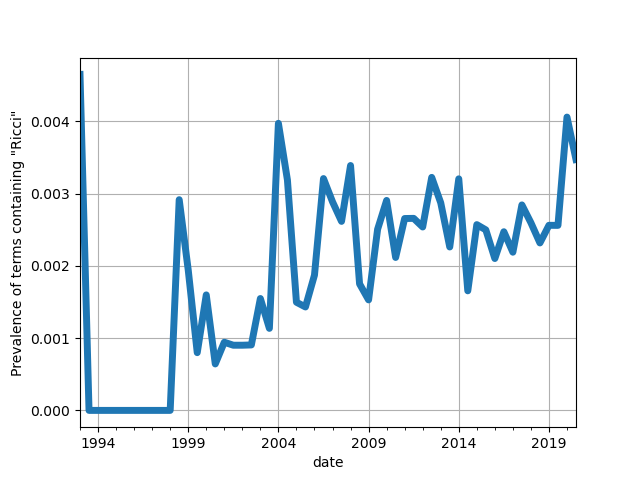
\includegraphics[width=0.85\textwidth]{../Images/ricci_preval.png}
            \end{center}
        \end{column}
    \end{columns}
\end{frame}

%%%%  FRAME  %%%%
\begin{frame}
    \frametitle{Información y Agradecimientos}
    \begin{columns}
        \begin{column}{0.6\textwidth}
            Esta trabajo comenzo como parte del \textbf{Formal Abstracts Project}.
        \end{column}
        \begin{column}{0.4\textwidth}
            \begin{center}
                
\includegraphics[width=0.9\textwidth]{../Images/fabstracts2.png}
            \end{center}
        \end{column}
    \end{columns}
        \pause
        Todo el súpercomputo se realizó gracias al apoyo de \textbf{Neocortex} en el PSC 
            \begin{center}
                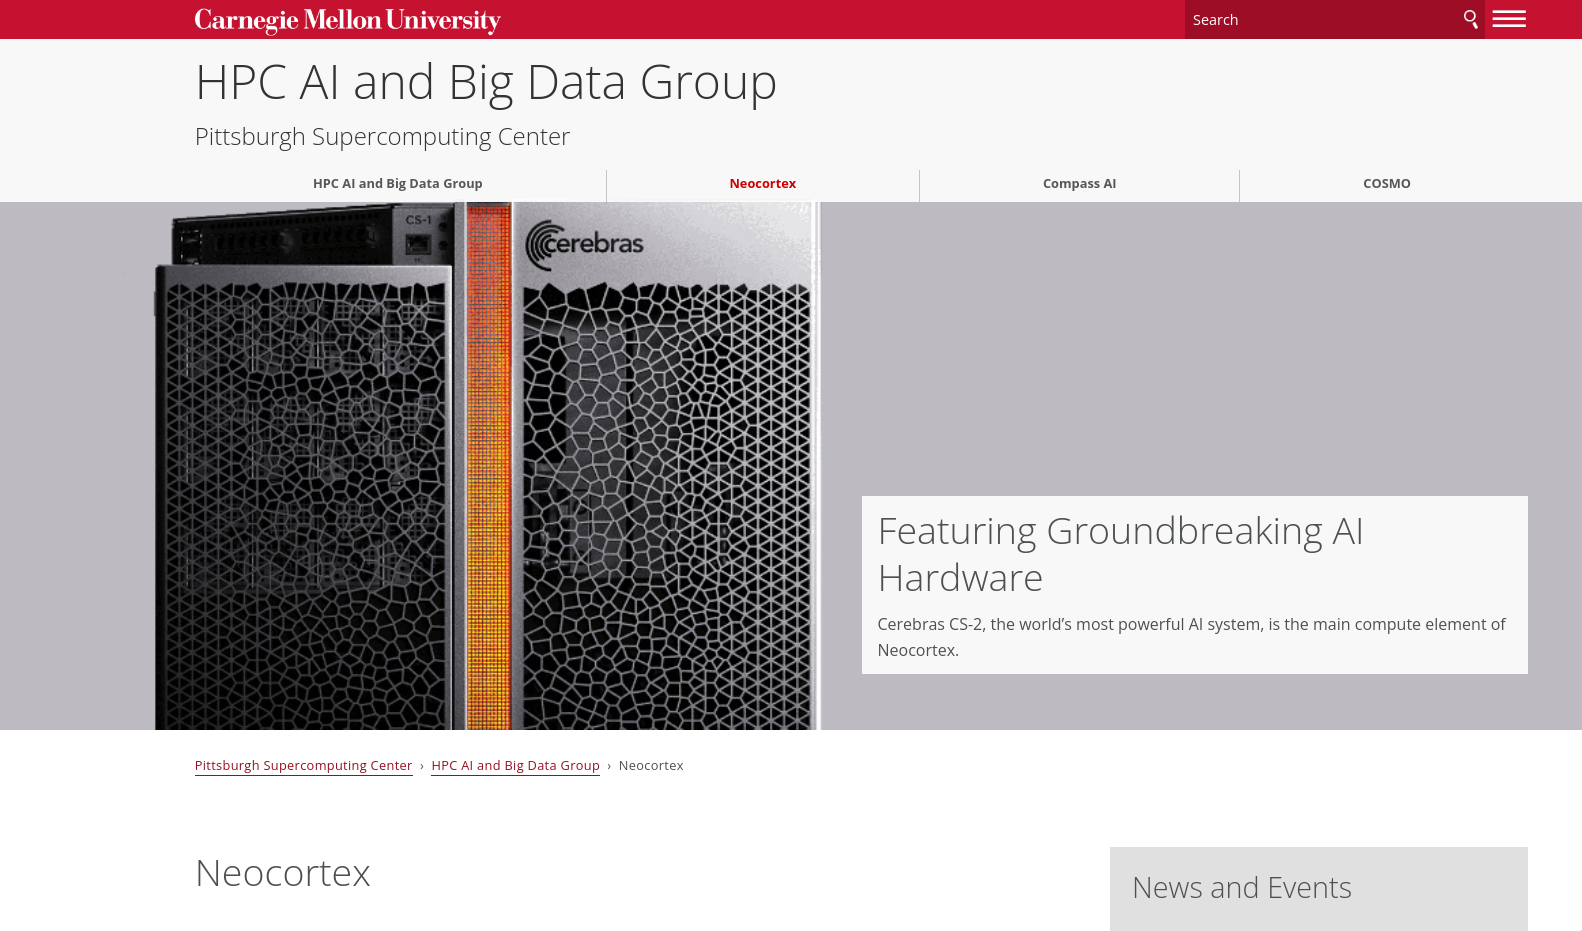
\includegraphics[width=0.8\textwidth]{../Images/neocortex_pic.png}
            \end{center}
\end{frame}

%%%%  FRAME  %%%%
\begin{frame}
    \frametitle{Trabajo para el futuro}
    \begin{itemize}
        \item Usar Zero-shot o RAG con los modelos más grandes.
            \note{Aunque no puede afinar (finetune) modelos de $\geq$ 70B de parametros,}
            \pause
        \item Esperar el ``port'' de modelos de Huggingface a Neocortex.
            \pause
        \item Dejar de usar preprocesadores del código fuente de \LaTeX{}.
    \end{itemize}
\end{frame}

\begin{frame}
\titlepage
\end{frame}
\end{document}
